
In the quench velocity-based approach, an electro-thermal element LINK68 is used to represent the composite strand, as discussed in Section~\ref{subsection:algorithms_geometry}. Figure~\ref{fig: q_vel_benchmarking_electrical_settings} illustrates additional initial and boundary conditions that allow for applying a power source identically to the standard analysis discussed in Section~\ref{section:quench_velocity_benchmarking_no_insulation_heat_balance}. The parameters related to the co-simulation in the quench velocity-based approach are shown in Table \ref{table: 1d_qv_benchmarking_geometry_parameters_quench_velocity}. 

\begin{figure}[H]
\centering
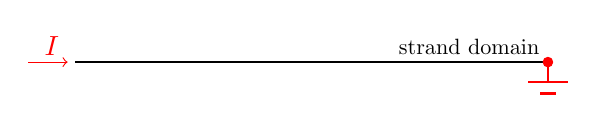
\begin{tikzpicture}[scale = 1]
\draw[thick, black] (-3,0) -- (3,0);
\filldraw[red] (3,0) circle (0.06);
\draw[thick, red] (3,0) -- (3,-0.25);
\draw[thick, red] (2.75,-0.25) -- (3.25,-0.25);
\draw[thick, red] (2.9,-0.4) -- (3.1,-0.4);
\draw[thin, red, ->] (-3.6,0) -- (-3.1,0);
\node[scale=0.8] at (2,0.2) {strand domain};
\node[scale=1.0, red] at (-3.3,0.2) {$I$};
\end{tikzpicture}
\caption{Electric boundary conditions.}
\label{fig: q_vel_benchmarking_electrical_settings}
\end{figure}

\begin{table}[H]
    \caption{Input parameters in the quench velocity-based approach.} 
    \vspace{-1.em} 
    \fontsize{10}{10}
    \selectfont 
    \renewcommand{\arraystretch}{1.5}
    \begin{center}
        \begin{tabular}{ ccc }  
        \hline
        parameter & value & unit \\
        \hline
        $t_\text{com}$ & 2.5 & [ms] \\
        $v_\text{quench, average}$ & 6.81 & [m/s] \\
        \hline 
        \end{tabular}
    \end{center}  
     \label{table: 1d_qv_benchmarking_geometry_parameters_quench_velocity} 
 \end{table}

First of all, the possibility of increasing the time step range is checked. Two time step ranges are chosen: $t_\text{step range} \in \{[0.01, 0.1], [0.1, 1]\}~\text{ms}$. In this comparison, the average quench velocity cannot be the condition statement corresponding to the relative error because it is an input parameter in the quench velocity-based approach. Therefore, the condition statement is based on the relative error of the resistive voltage with respect to the reference standard analysis. The results from two simulations having a different time step range, and relying on the quench velocity-based approach were compared with the reference solution. It appeared that the relative error remained below 0.1\% in both cases. Therefore, the time step range $t_\text{step range}=[0.1, 1]~\text{ms}$ is used in the quench velocity-based approach for the analysis of a bare strand, and with insulation and epoxy resin. In the analyses of a bare strand, the study over a 1 metre-long domain is conducted with a varying mesh size, $m=\{1, 2, 10, 20, 33.3\}~\text{mm}$. The geometric assumptions as well as the initial conditions are the same as in Section~\ref{section: 1D_quench_propagation_no_insulation}. As presented in Fig.~\ref{fig: q_vel_benchmarking_temp_distr_over_strand_no_insulation}, the quench velocity-based approach results in an underestimation of the nodal temperature along the strand. 

\begin{figure}[H]
\centering
    \begin{tikzpicture}
        \begin{axis}[
          no markers,
          width=0.7\linewidth, 
          height = 5.0cm,
          xlabel={$\bar{x},~\text{m}$},
          ylabel={$T,~\text{K}$},
          xmin=0.0,
          ymin=0.0,
          xmax=1.0,
          legend pos=outer north east
          ]
        %   Initial temperature curve for the mesh used in quench velocity modelling 
          \addplot[black] table[x=position,y=t_0,col sep=comma] {sections/q_vel_modelling_benchmarking/figures/results_no_insulation/quench_velocity_50_nodes_no_insulation.csv};
        %   Heat Balance Equation plots
          \addplot[red] table[x=position,y=t_0_03,col sep=comma] {sections/q_vel_modelling_benchmarking/figures/results_no_insulation/heat_balance_1000_nodes_benchmark.csv};
          \addplot[red] table[x=position,y=t_0_06,col sep=comma] {sections/q_vel_modelling_benchmarking/figures/results_no_insulation/heat_balance_1000_nodes_benchmark.csv};
          \addplot[red] table[x=position,y=t_0_1,col sep=comma] {sections/q_vel_modelling_benchmarking/figures/results_no_insulation/heat_balance_1000_nodes_benchmark.csv};
        %   Quench Velocity Modelling plots
          \addplot[blue] table[x=position,y=t_0_03,col sep=comma] {sections/q_vel_modelling_benchmarking/figures/results_no_insulation/quench_velocity_50_nodes_no_insulation.csv};
          \addplot[blue] table[x=position,y=t_0_06,col sep=comma] {sections/q_vel_modelling_benchmarking/figures/results_no_insulation/quench_velocity_50_nodes_no_insulation.csv};
          \addplot[blue] table[x=position,y=t_0_1,col sep=comma] {sections/q_vel_modelling_benchmarking/figures/results_no_insulation/quench_velocity_50_nodes_no_insulation.csv};
          \legend{
          $T_\text{init}$,
          standard,,,
          quench velocity
          }
        \end{axis}
        \draw[black, thick, ->] (2,3) -- (3,3);
        \node[scale = 1] at (3.8, 3) {$\vec{v}_\text{quench}$}; 
    \end{tikzpicture}
    \caption{Temperature distribution of the reference solution and the quench velocity-based approach with the mesh size of 20~mm for three time steps: $t=\{0.03, 0.06, 0.1\}$~s with a specified direction of quench velocity, $\vec{v}_\text{quench}$.}
    \label{fig: q_vel_benchmarking_temp_distr_over_strand_no_insulation}
\end{figure}

The reasons for the differences in the nodal temperature along the strand are twofold:
\begin{enumerate}
    \item In Fig.~\ref{fig:unidirectional_coupling_scheme}, in which the schematic of a one-directional coupling is presented, it is explained that the external routine updates resistive material properties at communication point $t_{j-1}$ and ANSYS solves the case for $t_{j}$. Therefore, the quenched zone is underestimated and 'delayed' with respect to the standard solution. Depending on the applied current and magnetic field to the model as well as the material properties of the geometry components, the error in the temperature distribution may stabilise or grow in time. To reduce this error, the number of communication points $t_\text{com}$ is increased to~40, which corresponds to a time window of $t=2.5~\text{ms}$. Nevertheless, this error is a natural consequence of applying the co-simulation.
    \item In the quench velocity-based approach, the material properties assignment to the strand is binary. The material has either resistive properties of the strand composite above its critical temperature or no resistance below this value. The transition region of a~current sharing temperature, being lower than the critical temperature, is not taken into account. The heat capacity of both Nb-Ti and copper is relatively low at critical temperatures. Therefore, even a small difference in heat deposition results in a~large temperature difference in the transition region.
\end{enumerate}

Not including the current sharing phenomenon in the standard analysis would reduce the discrepancy between two approaches during the benchmarking. However, the comparison of two analysis types aims at finding the maximum numerical error that the quench velocity-based approach gives. The study of separate factors, having an influence on the total discrepancy between the approaches, is not the goal of this chapter. As shown in Fig. \ref{fig: q_vel_modelling_res_volt_benchmarking}, the resistive voltage in the quench velocity-based approach follows the~curve of the standard solution. However, the resistive voltage is underestimated because the strand resistivity is a function of temperature, which is underestimated as well. 

\begin{figure}[H]
\centering
    \begin{tikzpicture}
        \begin{axis}[
          width=0.7\linewidth, 
          height = 4.0cm,
          xlabel={$t$, $\text{s}$},
          ylabel={$V_\text{res}$, $\text{V}$},
          xticklabel style={/pgf/number format/fixed},
          yticklabel style={/pgf/number format/fixed},
          xmin=0.0,
          xmax=0.1,
          legend pos=outer north east
          ]
          \addplot[red] table[x=time,y=heat_balance_benchmark,col sep=comma] {sections/q_vel_modelling_benchmarking/figures/results_no_insulation/quench_velocity_res_volt_benchmarking.csv};
          \addplot[blue, mark=*] table[x=time,y=50_nodes_quench_velocity,col sep=comma] {sections/q_vel_modelling_benchmarking/figures/results_no_insulation/quench_velocity_res_volt_benchmarking.csv};
          
          \legend{
          standard,
          quench velocity,
          }
          
        \end{axis}
    \end{tikzpicture}
    \caption{Comparison of the resistive voltage between the standard solution and the quench velocity-based approach with the mesh size of 20~mm.}
    \label{fig: q_vel_modelling_res_volt_benchmarking}
\end{figure}

Figures~\ref{fig: q_vel_modelling_res_volt_rel_error} and~\ref{fig: q_vel_modelling_hot_spot_rel_error} depict the evolution of the resistive voltage and the hot-spot temperature in time, respectively.
The longer the simulation lasts, the lower the relative error with respect to the reference solution in both cases becomes. One can observe that analysis with the mesh size of 1~mm also shows a similar evolution of the relative error. As the reference solution is characterised by the identical mesh size of 1~mm, the error cannot be explained by the decrease of mesh density, as presented in Fig.~\ref{fig: q_vel_modelling_energy_deposition}. This is due to the assumption of constant quench velocity which is not constant in the reference model. In fact, the quench propagation is a dynamic process which requires some time for the quench velocity to reach a steady-state value. To conclude, the error corresponding to the hot-spot temperature and the resistive voltage has to be accepted if one performs a simulation relying on the quench velocity-based approach.

\begin{figure}[H]
\centering
    \begin{tikzpicture}
        \begin{axis}[
          width=0.7\linewidth, 
          height = 4.0cm,
          xlabel={$t$, $\text{s}$},
          ylabel={$E_\text{r}$, \%},
          xticklabel style={/pgf/number format/fixed},
          xmin=0.0,
          xmax=0.1,
          legend pos=outer north east
          ]
          \addplot[blue, mark=*] table[x=time,y=50_nodes,col sep=comma] {sections/q_vel_modelling_benchmarking/figures/results_no_insulation/quench_velocity_res_volt_rel_error.csv};
          \addplot[red, mark=*] table[x=time,y=100_nodes,col sep=comma] {sections/q_vel_modelling_benchmarking/figures/results_no_insulation/quench_velocity_res_volt_rel_error.csv};
          \addplot[green, mark=*] table[x=time,y=1000_nodes,col sep=comma] {sections/q_vel_modelling_benchmarking/figures/results_no_insulation/quench_velocity_res_volt_rel_error.csv};
          \addlegendimage{/pgfplots/refstyle=plot_resistive_voltage}\addlegendentry{20~mm}
          \addlegendimage{/pgfplots/refstyle=plot_resistive_voltage}\addlegendentry{10~mm}
          \addlegendimage{/pgfplots/refstyle=plot_resistive_voltage}\addlegendentry{1~mm}
          
        \end{axis}
    \end{tikzpicture}
    \caption{Relative error of the resistive voltage for three different mesh sizes used for the quench velocity-based approach.}
    \label{fig: q_vel_modelling_res_volt_rel_error}
\end{figure}

\begin{figure}[H]
\centering
    \begin{tikzpicture}
        \begin{axis}[
          width=0.7\linewidth, 
          height = 4.0cm,
          xlabel={$t$, $\text{s}$},
          ylabel={$E_\text{r}$, \%},
          xticklabel style={/pgf/number format/fixed},
          xmin=0.0,
          xmax=0.1,
          legend pos=outer north east
          ]
          \addplot[blue, mark=*] table[x=time,y=50_nodes,col sep=comma] {sections/q_vel_modelling_benchmarking/figures/results_no_insulation/quench_velocity_hot_spot_rel_error.csv};
          \addplot[red, mark=*] table[x=time,y=100_nodes,col sep=comma] {sections/q_vel_modelling_benchmarking/figures/results_no_insulation/quench_velocity_hot_spot_rel_error.csv};
          \addplot[green, mark=*] table[x=time,y=1000_nodes,col sep=comma] {sections/q_vel_modelling_benchmarking/figures/results_no_insulation/quench_velocity_hot_spot_rel_error.csv};
          \addlegendimage{/pgfplots/refstyle=plot_resistive_voltage}\addlegendentry{20~mm}
          \addlegendimage{/pgfplots/refstyle=plot_resistive_voltage}\addlegendentry{10~mm}
          \addlegendimage{/pgfplots/refstyle=plot_resistive_voltage}\addlegendentry{1~mm}
          
        \end{axis}
    \end{tikzpicture}
    \caption{Relative error of the hot-spot temperature for three different mesh sizes used for the quench velocity-based approach.}
    \label{fig: q_vel_modelling_hot_spot_rel_error}
\end{figure}

